% ============================================================
%  第一章 矢量分析
%  内容依据谢树艺《工程数学 矢量分析与场论》
%  记号约定：变矢（矢性函数）用 \boldsymbol{}，
%            单位矢量 i/j/k 用 \mathbf{}
% ============================================================

\section{矢性函数的基本概念}

\textbf{常矢}：模和方向都不变的矢量。（零矢量方向任意，可以看作特殊的常矢。）

\textbf{变矢}：模和方向其中之一或都会改变的矢量。

\begin{definition}[矢性函数]
	设有数性变量 $t$ 和变矢 $\boldsymbol{A}$，如果对于 $t$ 在某个范围 $G$ 内的每一个数值，$\boldsymbol{A}$ 都以一个确定的矢量与它对应，则称 $\boldsymbol{A}$ 为数性变量 $t$ 的矢性函数，记作
	\begin{equation}
		\label{eq:基本概念:定义}
		\boldsymbol{A}=\boldsymbol{A}(t)
	\end{equation}
	并称 $G$ 为函数 $\boldsymbol{A}$ 的定义域。
\end{definition}

把矢性函数 $\boldsymbol{A}$ 沿坐标轴的三个方向分解，可得
\begin{equation}
	\label{eq:基本概念:坐标分解}
	\boldsymbol{A}=A_{x}(t)\,\mathbf{i}+A_{y}(t)\,\mathbf{j}+A_{z}(t)\,\mathbf{k}
\end{equation}

为了能用图形直观表示矢性函数 $\boldsymbol{A}(t)$ 的变化状态，把它的起点取在坐标原点，则终点 $M$ 描绘出一条曲线 $l$，称为矢性函数 $\boldsymbol{A}(t)$ 的\textbf{矢端曲线}，也称为 $\boldsymbol{A}$ 的\textbf{图形}；式~\eqref{eq:基本概念:坐标分解} 称为其矢量方程，如图~\ref{fig:矢端曲线} 所示。
\begin{figure}[htbp]
	\centering
	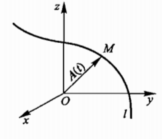
\includegraphics[width=0.45\textwidth]{../Figure/矢性函数的图形.png}
	\caption{矢性函数及其矢端曲线}
	\label{fig:矢端曲线}
\end{figure}

容易看到，矢端曲线的参数方程为
\begin{equation}
	\label{eq:基本概念:参数方程}
	x=A_{x}(t),\qquad y=A_{y}(t),\qquad z=A_{z}(t)
\end{equation}
显然，参数方程与矢量方程之间存在着一一对应关系。

\section{矢性函数的极限与连续性}

\begin{definition}[矢性函数的极限]
	设矢性函数 $\boldsymbol{A}(t)$ 在点 $t_{0}$ 的某个邻域内有定义（但在 $t_{0}$ 处可以没有定义），$\boldsymbol{A}_{0}$ 为一常矢。若对于任意给定的正数 $\varepsilon$，都存在正数 $\delta$，使当 $t$ 满足 $0<\left|t-t_{0}\right|<\delta$ 时，就有
	\begin{equation}
		\label{eq:极限:定义}
		\left|\boldsymbol{A}(t)-\boldsymbol{A}_{0}\right|<\varepsilon
	\end{equation}
	成立，则称 $\boldsymbol{A}_{0}$ 为矢性函数 $\boldsymbol{A}(t)$ 当 $t\rightarrow t_{0}$ 时的极限，记作
	\begin{equation}
		\label{eq:极限:记号}
		\lim_{t\rightarrow t_{0}}\boldsymbol{A}(t)=\boldsymbol{A}_{0}
	\end{equation}
\end{definition}

由此看出，矢性函数的极限具有与数性函数极限完全类似的运算法则。

\begin{definition}[矢性函数的连续性]
	若矢性函数 $\boldsymbol{A}(t)$ 在点 $t_{0}$ 的某个邻域内有定义，而且有
	\begin{equation}
		\label{eq:连续性:定义}
		\lim_{t\rightarrow t_{0}}\boldsymbol{A}(t)=\boldsymbol{A}\left(t_{0}\right)
	\end{equation}
	则称 $\boldsymbol{A}(t)$ 在 $t=t_{0}$ 处连续。
\end{definition}

显然，矢性函数 $\boldsymbol{A}(t)$ 在 $t_{0}$ 处连续 $\Leftrightarrow$ 三个坐标函数 $A_{x}(t),A_{y}(t),A_{z}(t)$ 在 $t_{0}$ 处连续。

\section{矢性函数的导数与微分}

\subsection{矢性函数的导数}

设有起点在 $O$ 点的矢性函数 $\boldsymbol{A}(t)$，当数性变量 $t$ 在其定义域内从 $t$ 变到 $t+\Delta t$（$\Delta t\neq 0$）时，对应的矢量分别为
\begin{equation}
	\label{eq:导数:端矢量}
	\boldsymbol{A}(t)=\overrightarrow{OM},\qquad
	\boldsymbol{A}(t+\Delta t)=\overrightarrow{ON}
\end{equation}
则 $\boldsymbol{A}(t+\Delta t)-\boldsymbol{A}(t)=\overrightarrow{MN}$ 叫做矢性函数 $\boldsymbol{A}(t)$ 的增量，记作 $\Delta\boldsymbol{A}$，即
\begin{equation}
	\label{eq:导数:增量}
	\Delta\boldsymbol{A}=\boldsymbol{A}(t+\Delta t)-\boldsymbol{A}(t)
\end{equation}
如图~\ref{fig:矢性函数的导数} 所示。
\begin{figure}[htbp]
	\centering
	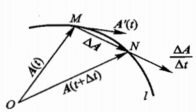
\includegraphics[width=0.5\textwidth]{../Figure/矢性函数的导数.png}
	\caption{矢性函数的增量与导矢}
	\label{fig:矢性函数的导数}
\end{figure}

由此可给出矢性函数的导数的定义。

\begin{definition}[矢性函数的导数]
	设矢性函数 $\boldsymbol{A}(t)$ 在点 $t$ 的某一邻域内有定义，并设 $t+\Delta t$ 也在这邻域内。若 $\boldsymbol{A}(t)$ 对应于 $\Delta t$ 的增量 $\Delta\boldsymbol{A}$ 与 $\Delta t$ 之比
	\begin{equation}
		\label{eq:导数:差商}
		\frac{\Delta\boldsymbol{A}}{\Delta t}
		=\frac{\boldsymbol{A}(t+\Delta t)-\boldsymbol{A}(t)}{\Delta t}
	\end{equation}
	在 $\Delta t\rightarrow 0$ 时其极限存在，则称此极限为矢性函数 $\boldsymbol{A}(t)$ 在点 $t$ 处的导数（简称导矢），记作 $\frac{\mathrm{d}\boldsymbol{A}}{\mathrm{d}t}$ 或 $\boldsymbol{A}^{\prime}(t)$，即
	\begin{equation}
		\label{eq:导数:定义}
		\frac{\mathrm{d}\boldsymbol{A}}{\mathrm{d}t}
		=\lim_{\Delta t\rightarrow 0}\frac{\Delta\boldsymbol{A}}{\Delta t}
		=\lim_{\Delta t\rightarrow 0}\frac{\boldsymbol{A}(t+\Delta t)-\boldsymbol{A}(t)}{\Delta t}
	\end{equation}
\end{definition}

若 $\boldsymbol{A}(t)$ 由坐标式~\eqref{eq:基本概念:坐标分解} 给出，且函数 $A_{x}(t),A_{y}(t),A_{z}(t)$ 在点 $t$ 可导，则有
\begin{equation}
	\label{eq:导数:坐标表示}
	\begin{aligned}
		\frac{\mathrm{d}\boldsymbol{A}}{\mathrm{d}t}
		&=\lim_{\Delta t\rightarrow 0}\frac{\Delta\boldsymbol{A}}{\Delta t}\\
		&=\lim_{\Delta t\rightarrow 0}\frac{\Delta A_{x}}{\Delta t}\,\mathbf{i}
		+\lim_{\Delta t\rightarrow 0}\frac{\Delta A_{y}}{\Delta t}\,\mathbf{j}
		+\lim_{\Delta t\rightarrow 0}\frac{\Delta A_{z}}{\Delta t}\,\mathbf{k}\\
		&=\frac{\mathrm{d}A_{x}}{\mathrm{d}t}\,\mathbf{i}
		+\frac{\mathrm{d}A_{y}}{\mathrm{d}t}\,\mathbf{j}
		+\frac{\mathrm{d}A_{z}}{\mathrm{d}t}\,\mathbf{k}
	\end{aligned}
\end{equation}
即 $\boldsymbol{A}^{\prime}(t)=A_{x}^{\prime}(t)\,\mathbf{i}+A_{y}^{\prime}(t)\,\mathbf{j}+A_{z}^{\prime}(t)\,\mathbf{k}$。此式把求矢性函数的导数归结为求三个数性函数的导数。

由几何上不难看出，导矢的几何意义为矢端曲线的切向矢量，指向 $t$ 值增大的一方。

\subsection{矢性函数的微分}

\begin{definition}[矢性函数的微分]
	设有矢性函数 $\boldsymbol{A}=\boldsymbol{A}(t)$，把
	\begin{equation}
		\label{eq:微分:定义}
		\mathrm{d}\boldsymbol{A}=\boldsymbol{A}^{\prime}(t)\,\mathrm{d}t
		\qquad(\mathrm{d}t=\Delta t)
	\end{equation}
	称为矢性函数 $\boldsymbol{A}(t)$ 在 $t$ 处的微分。
\end{definition}

几何意义如图~\ref{fig:矢性函数的微分} 所示。
\begin{figure}[htbp]
	\centering
	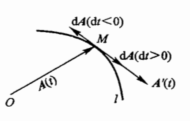
\includegraphics[width=0.5\textwidth]{../Figure/矢性函数的微分.png}
	\caption{矢性函数的微分}
	\label{fig:矢性函数的微分}
\end{figure}

微分的坐标表示式为
\begin{equation}
	\label{eq:微分:坐标表示}
	\begin{aligned}
		\mathrm{d}\boldsymbol{A}
		&=\boldsymbol{A}^{\prime}(t)\,\mathrm{d}t\\
		&=A_{x}^{\prime}(t)\,\mathrm{d}t\,\mathbf{i}
		+A_{y}^{\prime}(t)\,\mathrm{d}t\,\mathbf{j}
		+A_{z}^{\prime}(t)\,\mathrm{d}t\,\mathbf{k}
	\end{aligned}
\end{equation}
或
\begin{equation}
	\label{eq:微分:坐标表示形式2}
	\mathrm{d}\boldsymbol{A}=\mathrm{d}A_{x}\,\mathbf{i}+\mathrm{d}A_{y}\,\mathbf{j}+\mathrm{d}A_{z}\,\mathbf{k}
\end{equation}

\subsection{矢性函数的导数公式}

设矢性函数 $\boldsymbol{A}=\boldsymbol{A}(t)$、$\boldsymbol{B}=\boldsymbol{B}(t)$ 及数性函数 $u=u(t)$ 在 $t$ 的某个范围内可导，则下列公式在该范围内成立：
\begin{enumerate}
	\item $\dfrac{\mathrm{d}}{\mathrm{d}t}\boldsymbol{C}=\mathbf{0}$（$\boldsymbol{C}$ 为常矢）；
	\item $\dfrac{\mathrm{d}}{\mathrm{d}t}(\boldsymbol{A}\pm\boldsymbol{B})=\dfrac{\mathrm{d}\boldsymbol{A}}{\mathrm{d}t}\pm\dfrac{\mathrm{d}\boldsymbol{B}}{\mathrm{d}t}$；
	\item $\dfrac{\mathrm{d}}{\mathrm{d}t}(k\boldsymbol{A})=k\dfrac{\mathrm{d}\boldsymbol{A}}{\mathrm{d}t}$（$k$ 为常数）；
	\item $\dfrac{\mathrm{d}}{\mathrm{d}t}(u\boldsymbol{A})=\dfrac{\mathrm{d}u}{\mathrm{d}t}\boldsymbol{A}+u\dfrac{\mathrm{d}\boldsymbol{A}}{\mathrm{d}t}$；
	\item $\dfrac{\mathrm{d}}{\mathrm{d}t}(\boldsymbol{A}\cdot\boldsymbol{B})=\boldsymbol{A}\cdot\dfrac{\mathrm{d}\boldsymbol{B}}{\mathrm{d}t}+\dfrac{\mathrm{d}\boldsymbol{A}}{\mathrm{d}t}\cdot\boldsymbol{B}$，特例：$\dfrac{\mathrm{d}}{\mathrm{d}t}\boldsymbol{A}^{2}=2\boldsymbol{A}\cdot\dfrac{\mathrm{d}\boldsymbol{A}}{\mathrm{d}t}$（其中 $\boldsymbol{A}^{2}=\boldsymbol{A}\cdot\boldsymbol{A}$）；
	\item $\dfrac{\mathrm{d}}{\mathrm{d}t}(\boldsymbol{A}\times\boldsymbol{B})=\boldsymbol{A}\times\dfrac{\mathrm{d}\boldsymbol{B}}{\mathrm{d}t}+\dfrac{\mathrm{d}\boldsymbol{A}}{\mathrm{d}t}\times\boldsymbol{B}$；
	\item 复合函数求导公式：若 $\boldsymbol{A}=\boldsymbol{A}(u)$，$u=u(t)$，则
		\begin{equation}
			\label{eq:导数公式:复合函数}
			\frac{\mathrm{d}\boldsymbol{A}}{\mathrm{d}t}
			=\frac{\mathrm{d}\boldsymbol{A}}{\mathrm{d}u}\frac{\mathrm{d}u}{\mathrm{d}t}
		\end{equation}
\end{enumerate}

还有一些特殊的常见结论：
\begin{enumerate}
	\item 矢性函数 $\boldsymbol{A}(t)$ 的模不变的充要条件是 $\boldsymbol{A}\cdot\dfrac{\mathrm{d}\boldsymbol{A}}{\mathrm{d}t}=0$；
	\item 导矢的物理意义是末端点运动的速度（可由链式求导法则证明）。
\end{enumerate}

\section{矢性函数的积分}

\subsection{矢性函数的不定积分}

\begin{definition}[矢性函数的不定积分]
	若在 $t$ 的某个区间 $I$ 上，有 $\boldsymbol{B}^{\prime}(t)=\boldsymbol{A}(t)$，则称 $\boldsymbol{B}(t)$ 为 $\boldsymbol{A}(t)$ 在此区间上的一个原函数。在区间 $I$ 上，$\boldsymbol{A}(t)$ 的原函数的全体叫做 $\boldsymbol{A}(t)$ 在 $I$ 上的不定积分，记作
	\begin{equation}
		\label{eq:不定积分:定义}
		\int\boldsymbol{A}(t)\,\mathrm{d}t
	\end{equation}
\end{definition}

这个定义与数性函数的不定积分定义完全类似，故与数性函数一样，若已知 $\boldsymbol{B}(t)$ 是 $\boldsymbol{A}(t)$ 的一个原函数，则有
\begin{equation}
	\label{eq:不定积分:原函数}
	\int\boldsymbol{A}(t)\,\mathrm{d}t=\boldsymbol{B}(t)+\boldsymbol{C}
	\quad(\boldsymbol{C}\text{ 为任意常矢})
\end{equation}

而且，数性函数不定积分的基本性质对矢性函数来说也仍然成立。例如
\begin{equation}
	\label{eq:不定积分:线性性质}
	\begin{aligned}
		\int k\boldsymbol{A}(t)\,\mathrm{d}t &=k\int\boldsymbol{A}(t)\,\mathrm{d}t\\
		\int\left[\boldsymbol{A}(t)\pm\boldsymbol{B}(t)\right]\mathrm{d}t
		&=\int\boldsymbol{A}(t)\,\mathrm{d}t\pm\int\boldsymbol{B}(t)\,\mathrm{d}t\\
		\int u(t)\,\boldsymbol{a}\,\mathrm{d}t
		&=\boldsymbol{a}\int u(t)\,\mathrm{d}t
	\end{aligned}
\end{equation}
\begin{equation}
	\label{eq:不定积分:数积矢积性质}
	\begin{aligned}
		\int\boldsymbol{a}\cdot\boldsymbol{A}(t)\,\mathrm{d}t
		&=\boldsymbol{a}\cdot\int\boldsymbol{A}(t)\,\mathrm{d}t\\
		\int\boldsymbol{a}\times\boldsymbol{A}(t)\,\mathrm{d}t
		&=\boldsymbol{a}\times\int\boldsymbol{A}(t)\,\mathrm{d}t
	\end{aligned}
\end{equation}
其中 $k$ 为非零常数，$\boldsymbol{a}$ 为非零常矢。

据此，若已知 $\boldsymbol{A}=A_{x}(t)\,\mathbf{i}+A_{y}(t)\,\mathbf{j}+A_{z}(t)\,\mathbf{k}$，则由上述性质有
\begin{equation}
	\label{eq:不定积分:坐标表示}
	\int\boldsymbol{A}(t)\,\mathrm{d}t
	=\mathbf{i}\int A_{x}(t)\,\mathrm{d}t
	+\mathbf{j}\int A_{y}(t)\,\mathrm{d}t
	+\mathbf{k}\int A_{z}(t)\,\mathrm{d}t
\end{equation}
此式把求一个矢性函数的不定积分，归结为求三个数性函数的不定积分。

此外，数性函数的换元积分法与分部积分法亦适用于矢性函数。但由于两个矢量的矢量积服从负交换律，即 $\boldsymbol{A}\times\boldsymbol{B}=-(\boldsymbol{B}\times\boldsymbol{A})$，故其分部积分公式的右端应为两项相加
\begin{equation}
	\label{eq:不定积分:分部积分}
	\int\boldsymbol{A}\times\boldsymbol{B}^{\prime}\,\mathrm{d}t
	=\boldsymbol{A}\times\boldsymbol{B}+\int\boldsymbol{B}\times\boldsymbol{A}^{\prime}\,\mathrm{d}t
\end{equation}

\subsection{矢性函数的定积分}

\begin{definition}[矢性函数的定积分]
	设矢性函数 $\boldsymbol{A}(t)$ 在区间 $\left[T_{1},T_{2}\right]$ 上连续，则 $\boldsymbol{A}(t)$ 在 $\left[T_{1},T_{2}\right]$ 上的定积分是指下面形式的极限：
	\begin{equation}
		\label{eq:定积分:定义}
		\int_{T_{1}}^{T_{2}}\boldsymbol{A}(t)\,\mathrm{d}t
		=\lim_{\lambda\rightarrow 0}\sum_{i=1}^{n}\boldsymbol{A}\left(\xi_{i}\right)\Delta t_{i}
	\end{equation}
	其中 $T_{1}=t_{0}<t_{1}<t_{2}<\cdots<t_{n}=T_{2}$；$\xi_{i}$ 为区间 $\left[t_{i-1},t_{i}\right]$ 上的一点；$\Delta t_{i}=t_{i}-t_{i-1}$，$\lambda=\max\Delta t_{i}$，$i=1,2,\cdots,n$。
\end{definition}

可以看出，矢性函数的定积分概念也与数性函数的定积分完全类似，因此也具有和数性函数定积分相应的基本性质。例如：若 $\boldsymbol{B}(t)$ 是连续矢性函数 $\boldsymbol{A}(t)$ 在区间 $\left[T_{1},T_{2}\right]$ 上的一个原函数，则
\begin{equation}
	\label{eq:定积分:原函数}
	\int_{T_{1}}^{T_{2}}\boldsymbol{A}(t)\,\mathrm{d}t
	=\boldsymbol{B}\left(T_{2}\right)-\boldsymbol{B}\left(T_{1}\right)
\end{equation}
其他的性质就不再一一列举。
